\documentclass{extbook}[14pt]
\usepackage{multicol, enumerate, enumitem, hyperref, color, soul, setspace, parskip, fancyhdr, amssymb, amsthm, amsmath, bbm, latexsym, units, mathtools}
\everymath{\displaystyle}
\usepackage[headsep=0.5cm,headheight=0cm, left=1 in,right= 1 in,top= 1 in,bottom= 1 in]{geometry}
\usepackage{dashrule}  % Package to use the command below to create lines between items
\newcommand{\litem}[1]{\item #1

\rule{\textwidth}{0.4pt}}
\pagestyle{fancy}
\lhead{}
\chead{Answer Key for Progress Quiz 9 Version A}
\rhead{}
\lfoot{8590-6105}
\cfoot{}
\rfoot{Fall 2020}
\begin{document}
\textbf{This key should allow you to understand why you choose the option you did (beyond just getting a question right or wrong). \href{https://xronos.clas.ufl.edu/mac1105spring2020/courseDescriptionAndMisc/Exams/LearningFromResults}{More instructions on how to use this key can be found here}.}

\textbf{If you have a suggestion to make the keys better, \href{https://forms.gle/CZkbZmPbC9XALEE88}{please fill out the short survey here}.}

\textit{Note: This key is auto-generated and may contain issues and/or errors. The keys are reviewed after each exam to ensure grading is done accurately. If there are issues (like duplicate options), they are noted in the offline gradebook. The keys are a work-in-progress to give students as many resources to improve as possible.}

\rule{\textwidth}{0.4pt}

\begin{enumerate}\litem{
Solve the rational equation below. Then, choose the interval(s) that the solution(s) belongs to.
\[ \frac{5x}{7x + 5} + \frac{-4x^{2}}{-14x^{2} -59 x -35} = \frac{5}{-2x -7} \]

The solution is \( \text{There are two solutions: } x = -4.613 \text{ and } x = -0.387 \), which is option B.\begin{enumerate}[label=\Alph*.]
\item \( \text{All solutions lead to invalid or complex values in the equation.} \)


\item \( x_1 \in [-6.71, -4.31] \text{ and } x_2 \in [-0.57,-0.28] \)

* $x = -4.613 \text{ and } x = -0.387$, which is the correct option.
\item \( x \in [-3.61,-3.27] \)


\item \( x_1 \in [-6.71, -4.31] \text{ and } x_2 \in [-1,-0.57] \)


\item \( x \in [-1.16,0.71] \)


\end{enumerate}

\textbf{General Comment:} Distractors are different based on the number of solutions. Remember that after solving, we need to make sure our solution does not make the original equation divide by zero!
}
\litem{
Determine the domain of the function below.
\[ f(x) = \frac{3}{24x^{2} -56 x + 30} \]

The solution is \( \text{All Real numbers except } x = 0.833 \text{ and } x = 1.500. \), which is option B.\begin{enumerate}[label=\Alph*.]
\item \( \text{All Real numbers except } x = a, \text{ where } a \in [23.7, 25.5] \)

All Real numbers except $x = 24.000$, which corresponds to removing a distractor value from the denominator.
\item \( \text{All Real numbers except } x = a \text{ and } x = b, \text{ where } a \in [-0.8, 0.9] \text{ and } b \in [0.9, 3] \)

All Real numbers except $x = 0.833$ and $x = 1.500$, which is the correct option.
\item \( \text{All Real numbers except } x = a \text{ and } x = b, \text{ where } a \in [23.7, 25.5] \text{ and } b \in [29, 31.9] \)

All Real numbers except $x = 24.000$ and $x = 30.000$, which corresponds to not factoring the denominator correctly.
\item \( \text{All Real numbers except } x = a, \text{ where } a \in [-0.8, 0.9] \)

All Real numbers except $x = 0.833$, which corresponds to removing only 1 value from the denominator.
\item \( \text{All Real numbers.} \)

This corresponds to thinking the denominator has complex roots or that rational functions have a domain of all Real numbers.
\end{enumerate}

\textbf{General Comment:} Recall that dividing by zero is not a real number. Therefore the domain is all real numbers \textbf{except} those that make the denominator 0.
}
\litem{
Solve the rational equation below. Then, choose the interval(s) that the solution(s) belongs to.
\[ \frac{-36}{60x + 84} + 1 = \frac{-36}{60x + 84} \]

The solution is \( \text{all solutions are invalid or lead to complex values in the equation.} \), which is option A.\begin{enumerate}[label=\Alph*.]
\item \( \text{All solutions lead to invalid or complex values in the equation.} \)

*$x = -1.400$ leads to dividing by 0 in the original equation and thus is not a valid solution, which is the correct option.
\item \( x_1 \in [-3.4, -0.4] \text{ and } x_2 \in [0.4,2.4] \)

$x = -1.400 \text{ and } x = 1.400$, which corresponds to getting the correct solution and believing there should be a second solution to the equation.
\item \( x \in [-2.4,-0.4] \)

$x = -1.400$, which corresponds to not checking if this value leads to dividing by 0 in the original equation and thus is not a valid solution.
\item \( x \in [0.4,2.4] \)

$x = 1.400$, which corresponds to not distributing the factor $60x + 84$ correctly when trying to eliminate the fraction.
\item \( x_1 \in [-3.4, -0.4] \text{ and } x_2 \in [-3.4,0.6] \)

$x = -1.400 \text{ and } x = -1.400$, which corresponds to getting the correct solution and believing there should be a second solution to the equation.
\end{enumerate}

\textbf{General Comment:} Distractors are different based on the number of solutions. Remember that after solving, we need to make sure our solution does not make the original equation divide by zero!
}
\litem{
Solve the rational equation below. Then, choose the interval(s) that the solution(s) belongs to.
\[ \frac{42}{-30x + 24} + 1 = \frac{42}{-30x + 24} \]

The solution is \( \text{all solutions are invalid or lead to complex values in the equation.} \), which is option C.\begin{enumerate}[label=\Alph*.]
\item \( x \in [-0.2,1.8] \)

$x = 0.800$, which corresponds to not checking if this value leads to dividing by 0 in the original equation and thus is not a valid solution.
\item \( x \in [-1.5,-0.5] \)

$x = -0.800$, which corresponds to not distributing the factor $-30x + 24$ correctly when trying to eliminate the fraction.
\item \( \text{All solutions lead to invalid or complex values in the equation.} \)

*$x = 0.800$ leads to dividing by 0 in the original equation and thus is not a valid solution, which is the correct option.
\item \( x_1 \in [0.5, 1.3] \text{ and } x_2 \in [-1.2,2.8] \)

$x = 0.800 \text{ and } x = 0.800$, which corresponds to getting the correct solution and believing there should be a second solution to the equation.
\item \( x_1 \in [-1.5, -0.5] \text{ and } x_2 \in [-1.2,2.8] \)

$x = -0.800 \text{ and } x = 0.800$, which corresponds to getting the correct solution and believing there should be a second solution to the equation.
\end{enumerate}

\textbf{General Comment:} Distractors are different based on the number of solutions. Remember that after solving, we need to make sure our solution does not make the original equation divide by zero!
}
\litem{
Choose the graph of the equation below.
\[ f(x) = \frac{-1}{x - 3} - 1 \]

The solution is the graph below, which is option E.
\begin{center}
    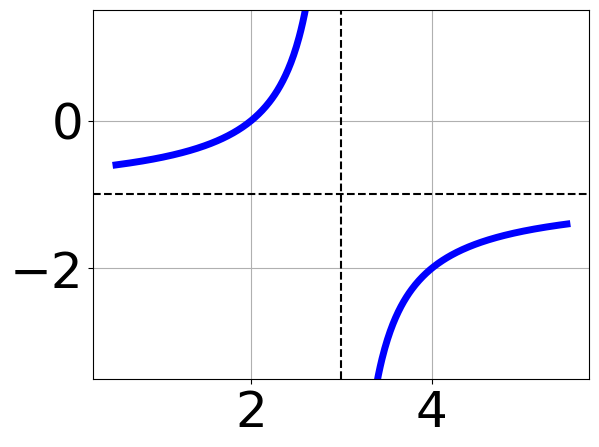
\includegraphics[width=0.3\textwidth]{../Figures/rationalEquationToGraphCopyEA.png}
\end{center}\begin{enumerate}[label=\Alph*.]
\begin{multicols}{2}
\item 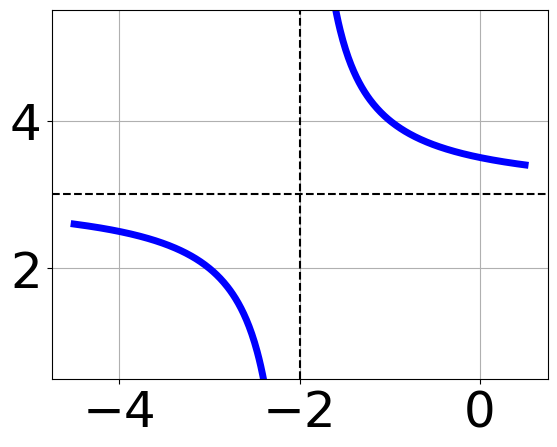
\includegraphics[width = 0.3\textwidth]{../Figures/rationalEquationToGraphCopyAA.png}
\item 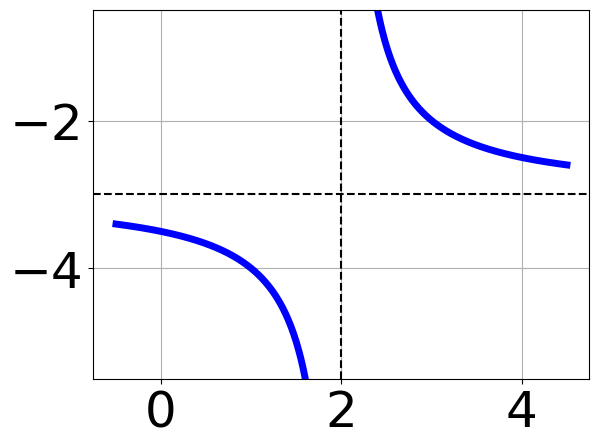
\includegraphics[width = 0.3\textwidth]{../Figures/rationalEquationToGraphCopyBA.png}
\item 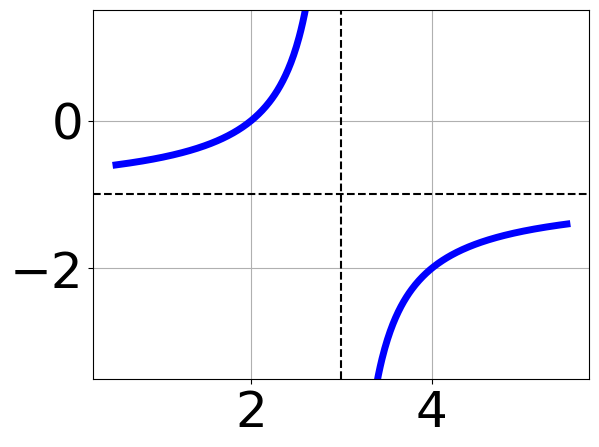
\includegraphics[width = 0.3\textwidth]{../Figures/rationalEquationToGraphCopyCA.png}
\item 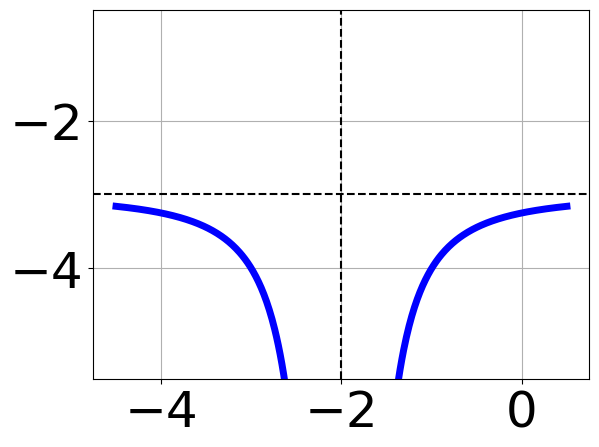
\includegraphics[width = 0.3\textwidth]{../Figures/rationalEquationToGraphCopyDA.png}
\end{multicols}\item None of the above.\end{enumerate}
\textbf{General Comment:} Remember that the general form of a basic rational equation is $ f(x) = \frac{a}{(x-h)^n} + k$, where $a$ is the leading coefficient (and in this case, we assume is either $1$ or $-1$), $n$ is the degree (in this case, either $1$ or $2$), and $(h, k)$ is the intersection of the asymptotes.
}
\litem{
Determine the domain of the function below.
\[ f(x) = \frac{6}{12x^{2} +29 x + 15} \]

The solution is \( \text{All Real numbers except } x = -1.667 \text{ and } x = -0.750. \), which is option E.\begin{enumerate}[label=\Alph*.]
\item \( \text{All Real numbers except } x = a, \text{ where } a \in [-16.7, -14.9] \)

All Real numbers except $x = -15.000$, which corresponds to removing a distractor value from the denominator.
\item \( \text{All Real numbers except } x = a \text{ and } x = b, \text{ where } a \in [-16.7, -14.9] \text{ and } b \in [-12.3, -11.6] \)

All Real numbers except $x = -15.000$ and $x = -12.000$, which corresponds to not factoring the denominator correctly.
\item \( \text{All Real numbers.} \)

This corresponds to thinking the denominator has complex roots or that rational functions have a domain of all Real numbers.
\item \( \text{All Real numbers except } x = a, \text{ where } a \in [-4, -1.5] \)

All Real numbers except $x = -1.667$, which corresponds to removing only 1 value from the denominator.
\item \( \text{All Real numbers except } x = a \text{ and } x = b, \text{ where } a \in [-4, -1.5] \text{ and } b \in [-1.6, 0.1] \)

All Real numbers except $x = -1.667$ and $x = -0.750$, which is the correct option.
\end{enumerate}

\textbf{General Comment:} Recall that dividing by zero is not a real number. Therefore the domain is all real numbers \textbf{except} those that make the denominator 0.
}
\litem{
Choose the equation of the function graphed below.

\begin{center}
    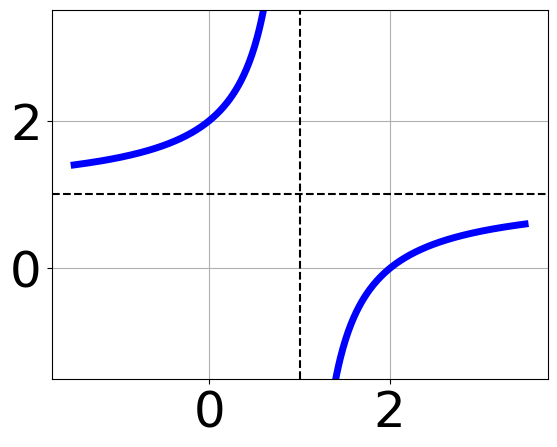
\includegraphics[width=0.5\textwidth]{../Figures/rationalGraphToEquationCopyA.png}
\end{center}




The solution is \( \text{None of the above as it should be } f(x) = \frac{1}{x + 2} - 3 \), which is option E.\begin{enumerate}[label=\Alph*.]
\item \( f(x) = \frac{-1}{(x - 2)^2} - 7 \)

Corresponds to thinking the graph was a shifted version of $\frac{1}{x^2}$, using the general form $f(x) = \frac{a}{x+h}+k$, the opposite leading coefficient, AND not noticing the $y$-value was wrong.
\item \( f(x) = \frac{1}{(x + 2)^2} - 7 \)

Corresponds to thinking the graph was a shifted version of $\frac{1}{x^2}$ not noticing the $y$-value was wrong.
\item \( f(x) = \frac{1}{x + 2} - 7 \)

The $y$-value of the equation does not match the graph.
\item \( f(x) = \frac{-1}{x - 2} - 7 \)

Corresponds to using the general form $f(x) = \frac{a}{x+h}+k$, the opposite leading coefficient AND not noticing the $y$-value was wrong.
\item \( \text{None of the above} \)

None of the equation options were the correct equation.
\end{enumerate}

\textbf{General Comment:} Remember that the general form of a basic rational equation is $ f(x) = \frac{a}{(x-h)^n} + k$, where $a$ is the leading coefficient (and in this case, we assume is either $1$ or $-1$), $n$ is the degree (in this case, either $1$ or $2$), and $(h, k)$ is the intersection of the asymptotes.
}
\litem{
Choose the equation of the function graphed below.

\begin{center}
    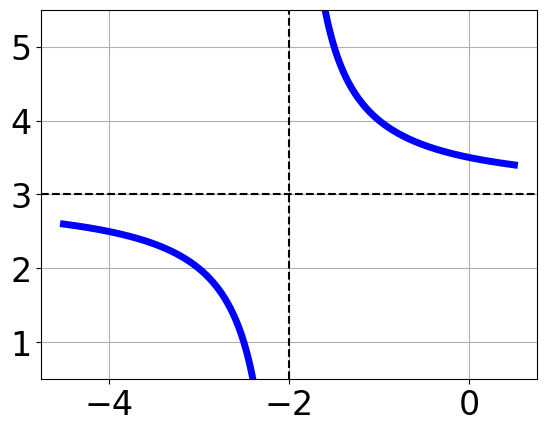
\includegraphics[width=0.5\textwidth]{../Figures/rationalGraphToEquationA.png}
\end{center}




The solution is \( \text{None of the above as it should be } f(x) = \frac{-1}{(x + 3)^2} - 1 \), which is option E.\begin{enumerate}[label=\Alph*.]
\item \( f(x) = \frac{1}{(x + 3)^2} - 1 \)

Corresponds to using the general form $f(x) = \frac{a}{(x-h)^2}+k$ and the opposite leading coefficient.
\item \( f(x) = \frac{-1}{(x - 3)^2} - 1 \)

The $x$-value of the equation does not match the graph.
\item \( f(x) = \frac{1}{x + 3} - 1 \)

Corresponds to thinking the graph was a shifted version of $\frac{1}{x}$, using the general form $f(x) = \frac{a}{(x-h)^2}+k$, and the opposite leading coefficient.
\item \( f(x) = \frac{-1}{x - 3} - 1 \)

Corresponds to thinking the graph was a shifted version of $\frac{1}{x}$.
\item \( \text{None of the above} \)

None of the equation options were the correct equation.
\end{enumerate}

\textbf{General Comment:} Remember that the general form of a basic rational equation is $ f(x) = \frac{a}{(x-h)^n} + k$, where $a$ is the leading coefficient (and in this case, we assume is either $1$ or $-1$), $n$ is the degree (in this case, either $1$ or $2$), and $(h, k)$ is the intersection of the asymptotes.
}
\litem{
Choose the graph of the equation below.
\[ f(x) = \frac{-1}{x + 3} - 1 \]

The solution is the graph below, which is option E.
\begin{center}
    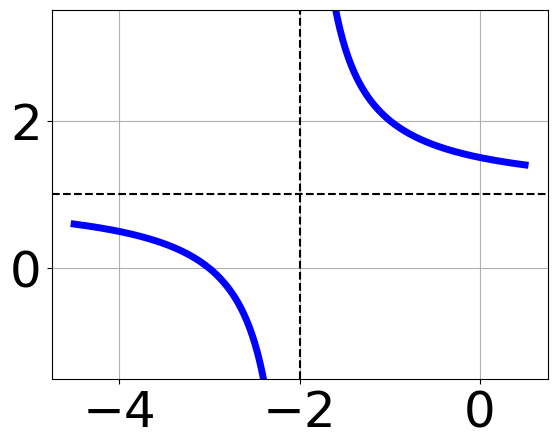
\includegraphics[width=0.3\textwidth]{../Figures/rationalEquationToGraphEA.png}
\end{center}\begin{enumerate}[label=\Alph*.]
\begin{multicols}{2}
\item 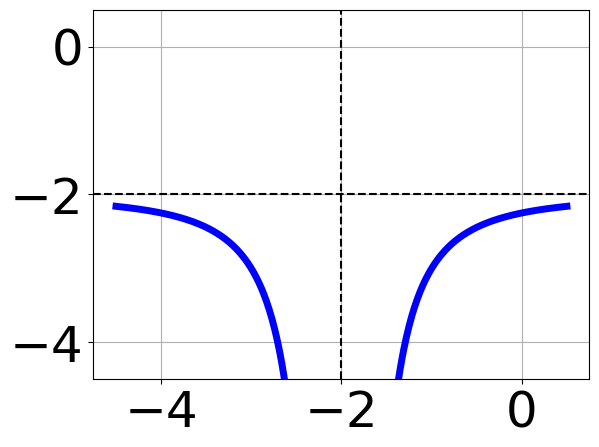
\includegraphics[width = 0.3\textwidth]{../Figures/rationalEquationToGraphAA.png}
\item 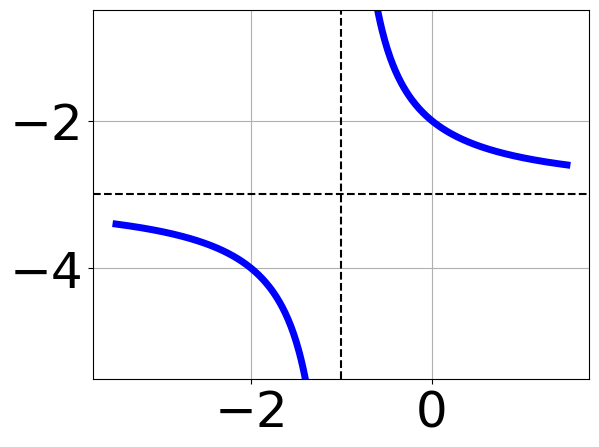
\includegraphics[width = 0.3\textwidth]{../Figures/rationalEquationToGraphBA.png}
\item 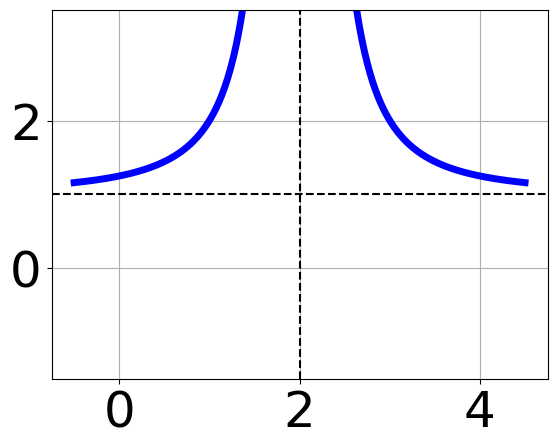
\includegraphics[width = 0.3\textwidth]{../Figures/rationalEquationToGraphCA.png}
\item 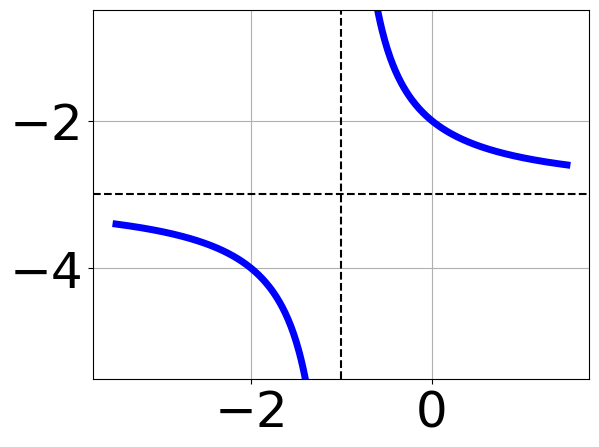
\includegraphics[width = 0.3\textwidth]{../Figures/rationalEquationToGraphDA.png}
\end{multicols}\item None of the above.\end{enumerate}
\textbf{General Comment:} Remember that the general form of a basic rational equation is $ f(x) = \frac{a}{(x-h)^n} + k$, where $a$ is the leading coefficient (and in this case, we assume is either $1$ or $-1$), $n$ is the degree (in this case, either $1$ or $2$), and $(h, k)$ is the intersection of the asymptotes.
}
\litem{
Solve the rational equation below. Then, choose the interval(s) that the solution(s) belongs to.
\[ \frac{-2x}{-2x + 6} + \frac{-3x^{2}}{-12x^{2} +22 x + 42} = \frac{-4}{6x + 7} \]

The solution is \( \text{There are two solutions: } x = 0.729 \text{ and } x = -2.195 \), which is option B.\begin{enumerate}[label=\Alph*.]
\item \( x \in [-2.01,-0.52] \)


\item \( x_1 \in [0.05, 1.45] \text{ and } x_2 \in [-3.2,-0.8] \)

* $x = 0.729 \text{ and } x = -2.195$, which is the correct option.
\item \( x \in [-3.39,-1.71] \)


\item \( \text{All solutions lead to invalid or complex values in the equation.} \)


\item \( x_1 \in [0.05, 1.45] \text{ and } x_2 \in [-1.6,4.7] \)


\end{enumerate}

\textbf{General Comment:} Distractors are different based on the number of solutions. Remember that after solving, we need to make sure our solution does not make the original equation divide by zero!
}
\end{enumerate}

\end{document}